\chapter{Manipulação de Imagens (2D)}

\section{Reconstrução Multiplanar}

Ao importar as imagens, o InVesalius mostra, automaticamente, a sua reconstrução
multiplanar nas orientações Axial, Sagital e Coronal, bem como uma janela para manipulação 3D.
Veja a figura \ref{fig:mpr}.

\begin{figure}[!htb]
\centering
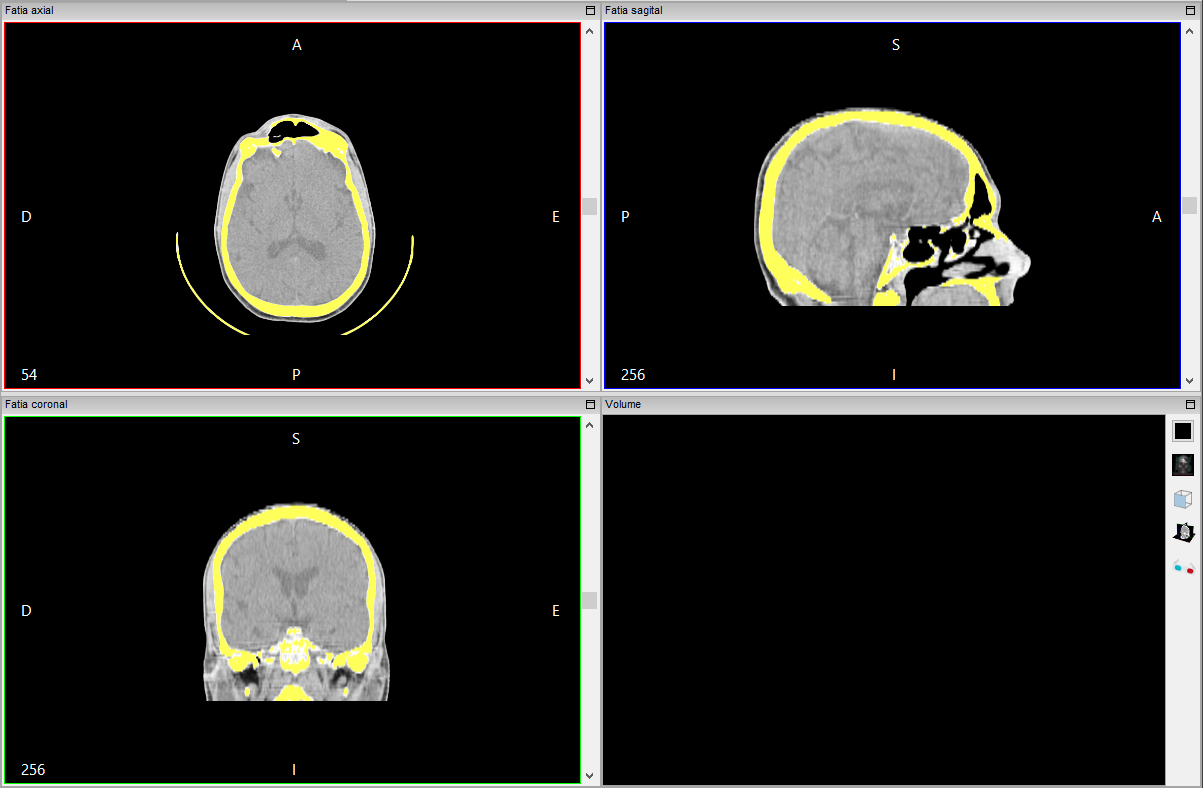
\includegraphics[scale=0.30]{multiplanar_mask_window_pt.png}
\caption{Reconstrução multiplanar}
\label{fig:mpr}
\end{figure}

\newpage

Além de criar a reconstrução multiplanar, o InVesalius segmenta a imagem, destacando, por exemplo, os
ossos dos tecidos moles. O destaque é representado por meio da aplicação de cores sobre a estrutura
segmentada, isto é, as cores formam uma máscara sobre a imagem destacando a estrutura (figura
\ref{fig:mpr}). Isso será discutido em mais detalhes nos próximos capítulos.

Para esconder a máscara, usa-se o gerenciador de dados, localizado no canto inferior esquerdo
da tela. Basta escolher a aba \textbf{Máscaras} e clicar \textbf{uma} vez com o botão
\textbf{esquerdo} do mouse sobre o ícone do olho ao lado de \textbf{"Máscara 1"}. Veja a figura
\ref{fig:ger_masc}.

\begin{figure}[!htb]
\centering
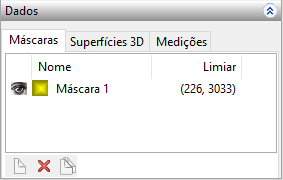
\includegraphics[scale=0.8]{data_mask_pt.png}
\caption{Gerenciador de máscaras}
\label{fig:ger_masc}
\end{figure}

O ícone do olho desaparece, e as cores da máscara de segmentação são escondidas (figura
\ref{fig:mpr_sem_mask}).

\begin{figure}[!htb]
\centering
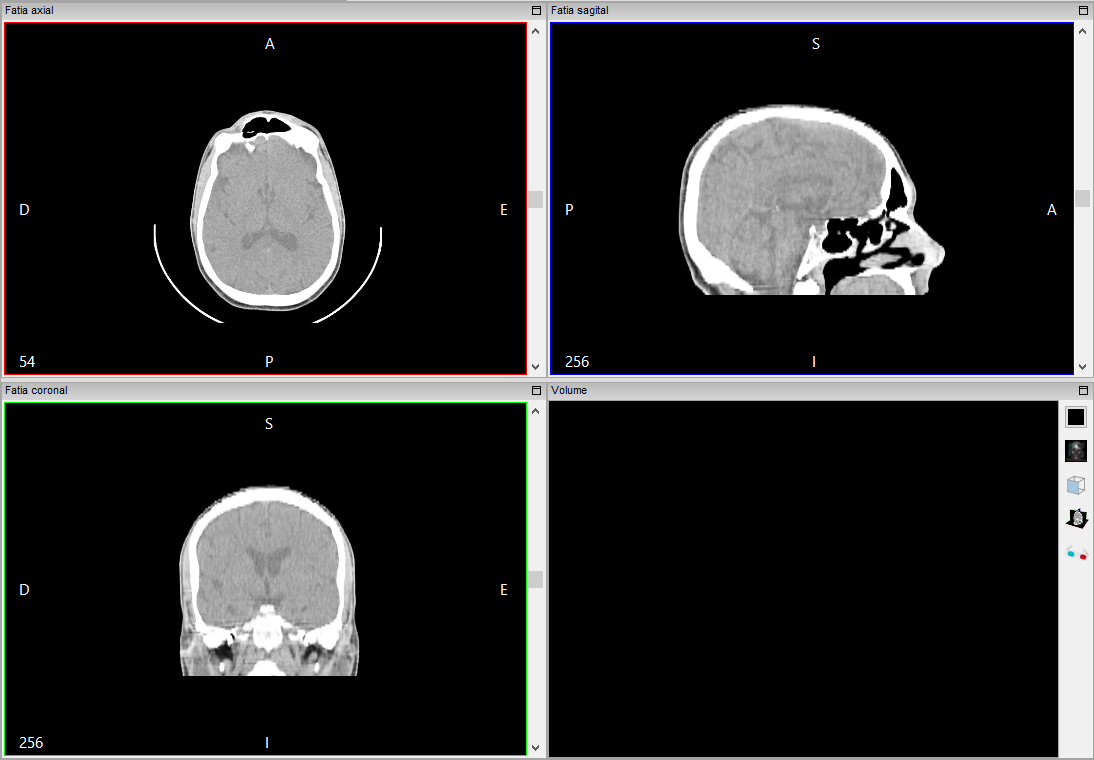
\includegraphics[scale=0.30]{multiplanar_window_pt.png}
\caption{Reconstrução multiplanar sem máscara de segmentação}
\label{fig:mpr_sem_mask}
\end{figure}

\subsection{Orientação axial}

A orientação axial é composta de cortes transversais da região
de interesse, ou seja, cortes paralelos ao plano axial do corpo humano.
Na figura \ref{fig:axial_corte}, é exibida uma imagem em orientação axial da
região do crânio.

\begin{figure}[!htb]
\centering
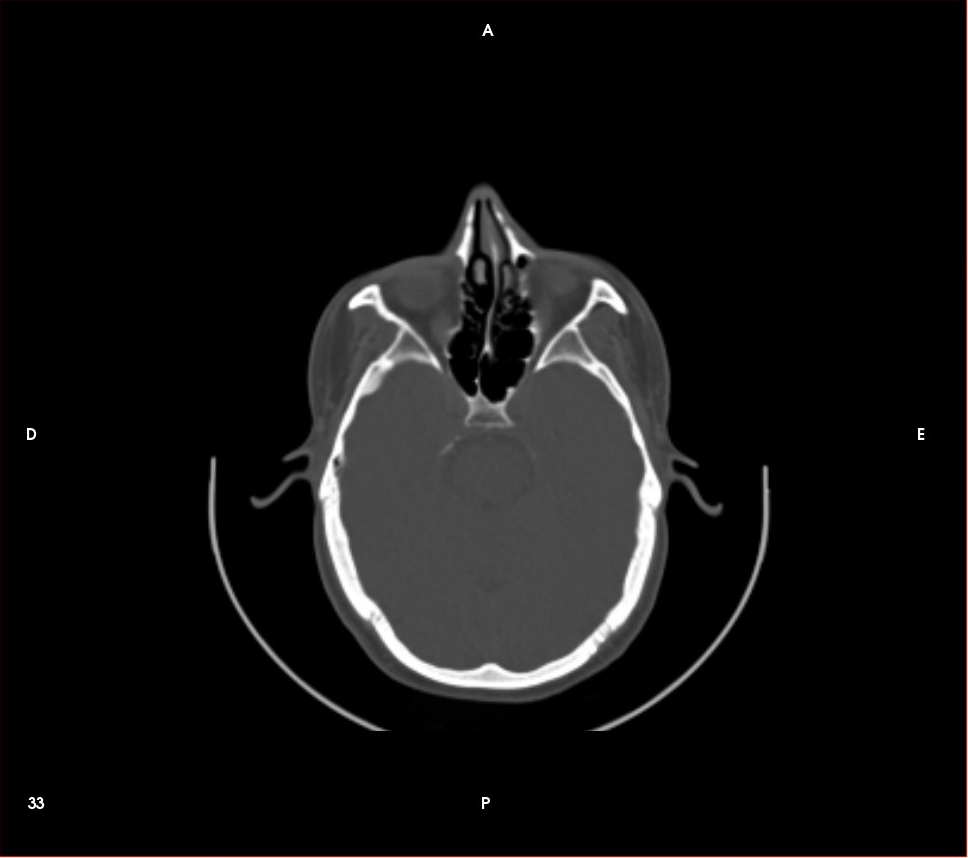
\includegraphics[scale=0.15]{axial.jpg}
\caption{Corte axial}
\label{fig:axial_corte}
\end{figure}

\subsection{Orientação sagital}

A orientação sagital é composta de cortes realizados lateralmente
em relação à região de interesse, ou seja, cortes paralelos ao plano sagital do corpo humano,
que o divide nas porções esquerda e direita.
A figura \ref{fig:sagital_slice} mostra uma imagem do crânio em orientação sagital.

\begin{figure}[!htb]
\centering
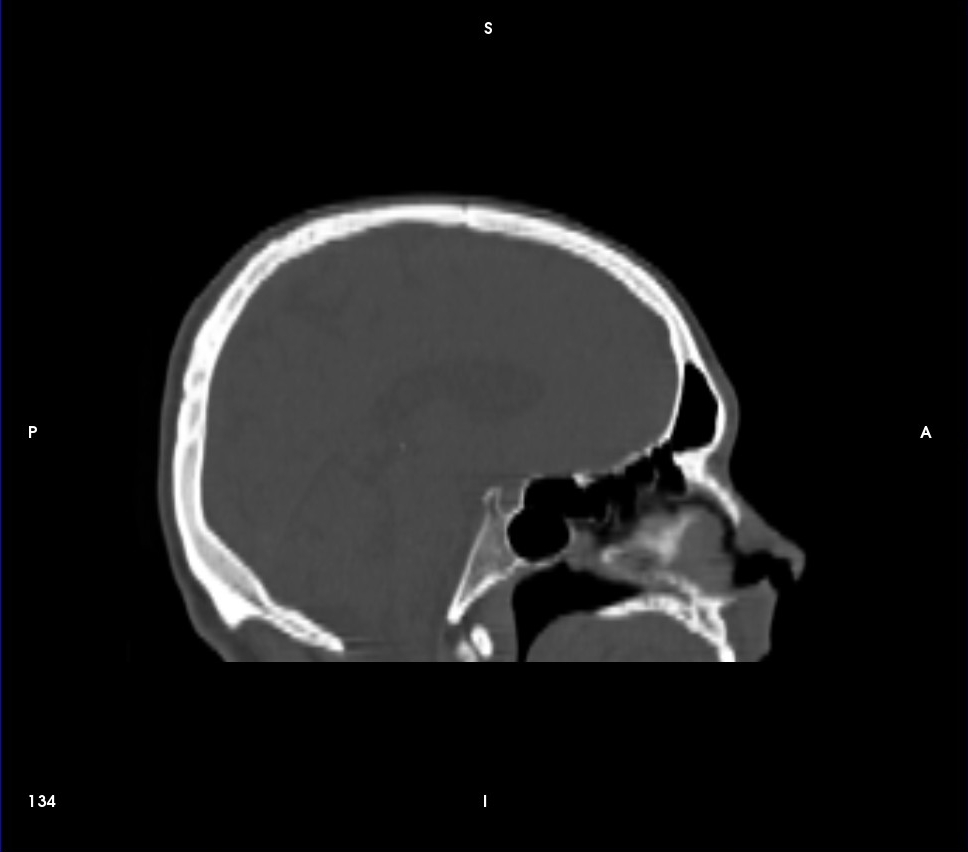
\includegraphics[scale=0.15]{sagital.jpg}
\caption{Corte sagital}
\label{fig:sagital_slice}
\end{figure}

\newpage

\subsection{Orientação coronal}

A orientação coronal é composta de cortes paralelos ao plano coronal,
que divide o corpo humano em metades ventral e dorsal.
A figura \ref{fig:coronal_slice} mostra uma imagem do crânio em orientação
coronal.

\begin{figure}[!htb]
\centering
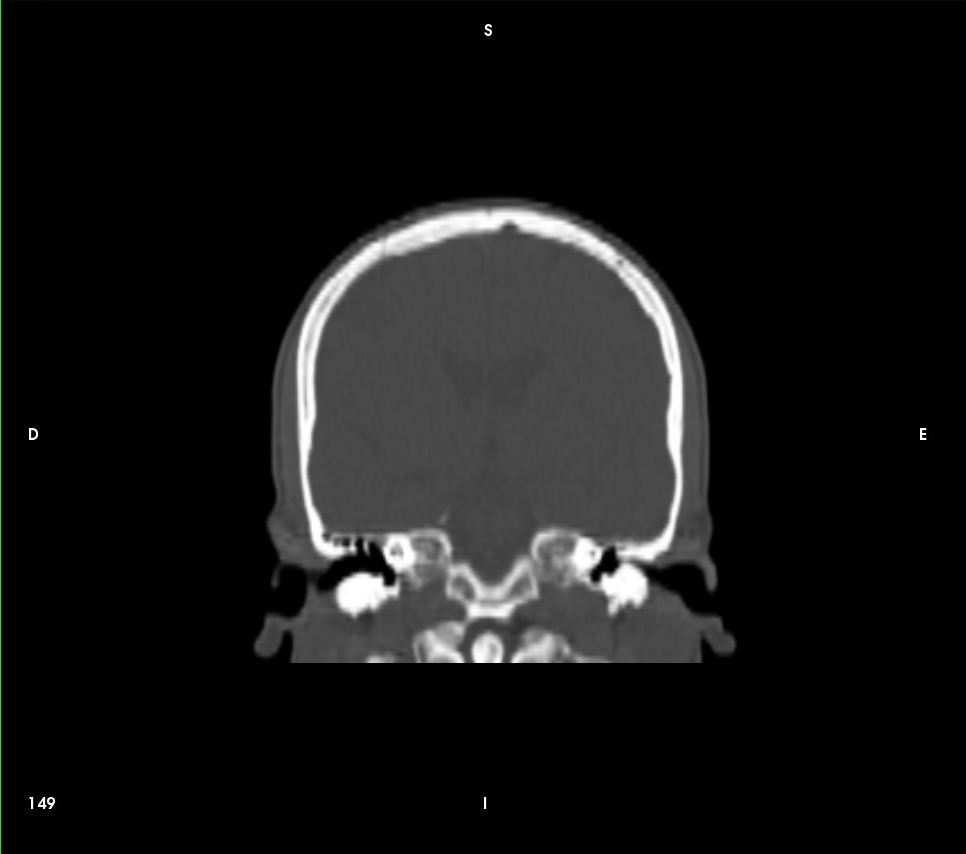
\includegraphics[scale=0.15]{coronal.jpg}
\caption{Corte coronal}
\label{fig:coronal_slice}
\end{figure}


\section{Correspondência entre as orientações axial, sagital e coronal}

Para saber qual o ponto comum das imagens nas diferentes orientações, basta acionar o
recurso "Cruz de interseção de fatias" pelo ícone de atalho localizado na barra de ferramentas.
Veja a figura \ref{fig:cross_icon}.

\begin{figure}[!htb]
\centering

\includegraphics[scale=1]{cross.png}
\caption{Atalho para mostrar ponto comum entre diferentes orientações}
\label{fig:cross_icon}
\end{figure}

Quando o recurso é acionado, dois segmentos de reta que se cruzam perpendicularmente são exibidos
sobre cada imagem (figura \ref{fig:cross_all}). O ponto de interseção de cada par de segmentos
representa o ponto comum  entre as diferentes orientações.

\newpage

Para modificar o ponto, mantenha \textbf{pressionado} o botão \textbf{esquerdo} do mouse e o
\textbf{arraste}. Automaticamente, os pontos correspondentes serão atualizados em cada imagem.

\begin{figure}[!htb]
\centering
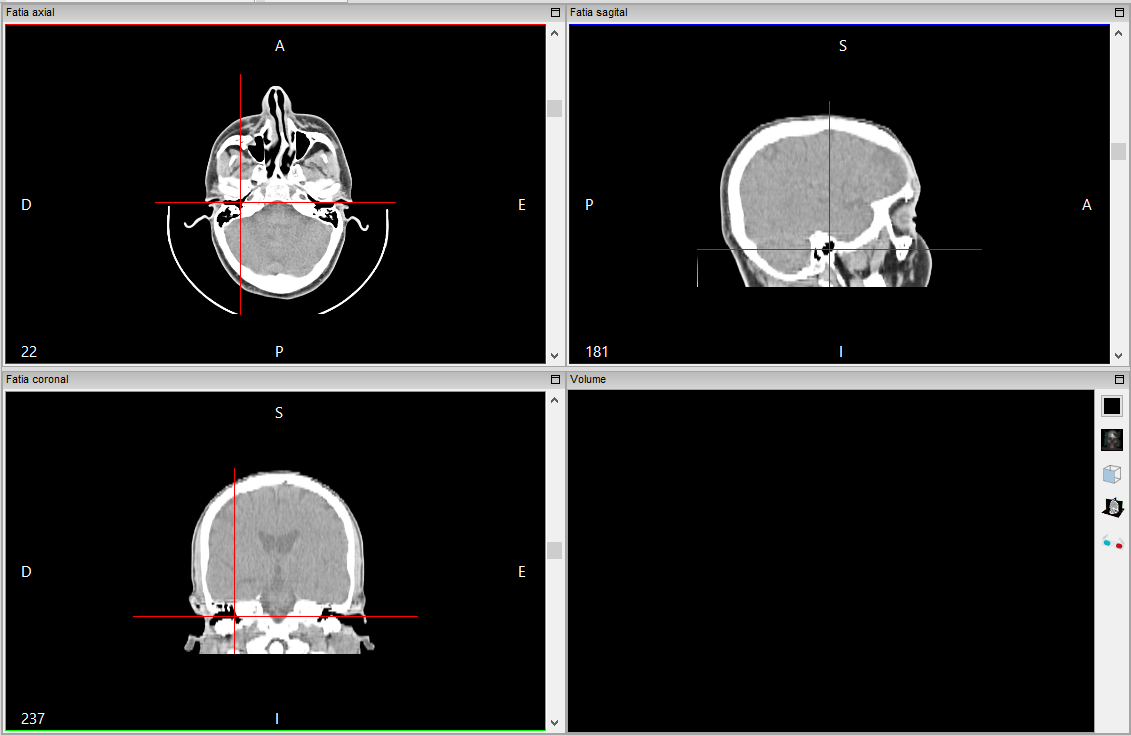
\includegraphics[scale=0.4]{multiplanar_window_cross_pt.png}
\caption{Ponto comum entre orientações diferentes}
\label{fig:cross_all}
\end{figure}

Para desativar a funcionalidade, basta clicar novamente sobre o atalho (figura \ref{fig:cross_icon}).
Esse recurso pode ser utilizado em conjunto com o editor de fatias (que será comentado mais à frente).

\newpage

\section{Mover}

Para mover uma imagem na tela, pode-se utilizar o ícone do atalho "Mover" da barra de ferramentas (figura
\ref{fig:move_icon}). Clique sobre o ícone para ativar o recurso e, em seguida, com o botão
\textbf{esquerdo} do mouse pressionado sobre a imagem, \textbf{arraste-a} para a direção desejada.
A figura \ref{fig:move_img} mostra uma imagem deslocada (movida).

\begin{figure}[!htb]
\centering

\includegraphics[scale=0.25]{tool_translate_original.png}
\caption{Atalho para mover imagens}
\label{fig:move_icon}
\end{figure}

\begin{figure}[!htb]
\centering
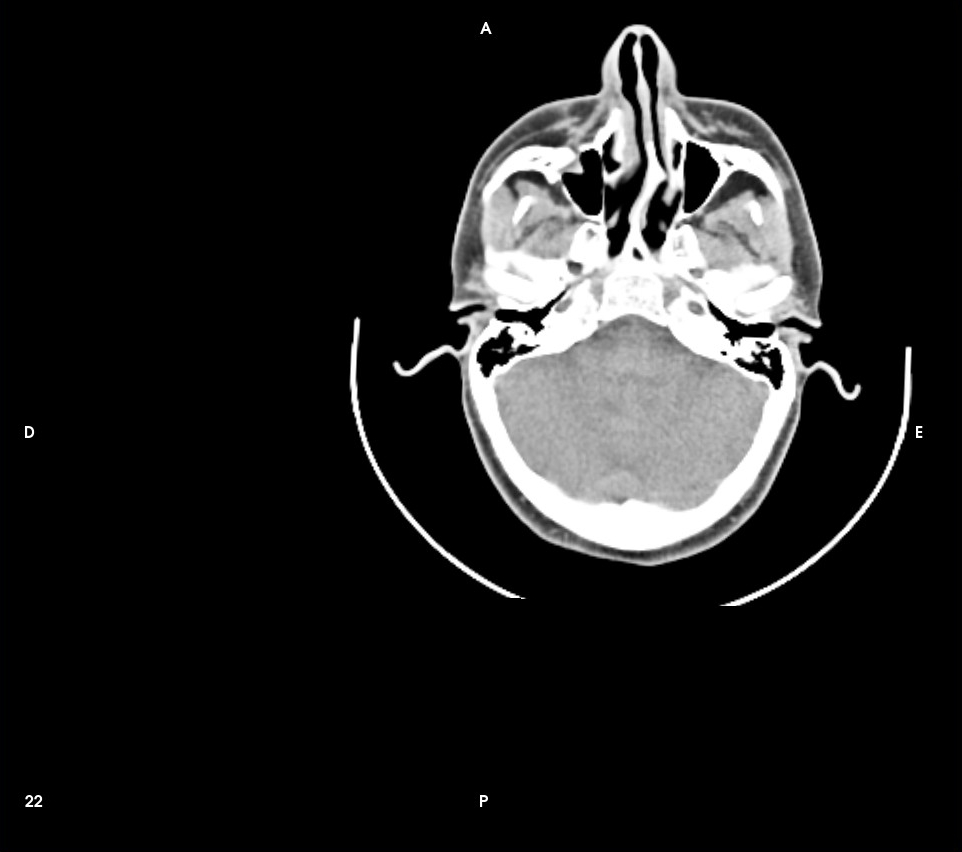
\includegraphics[scale=0.25]{axial_pan.jpg}
\caption{Imagem deslocada}
\label{fig:move_img}
\end{figure}

\section{Rotacionar}

A rotação de imagens pode ser ativada pelo ícone do atalho "Rotacionar" da barra de ferramentas (figura
\ref{fig:rot_icon}). Para rotacionar uma imagem, clique sobre o ícone e, em seguida, com o botão
\textbf{esquerdo} do mouse pressionado sobre a imagem, \textbf{arraste-a} no sentido horário ou
anti-horário, dependendo do sentido de rotação desejado.

\begin{figure}[!htb]
\centering

\includegraphics[scale=0.25]{tool_rotate_original.png}
\caption{Atalho para rotacionar imagens}
\label{fig:rot_icon}
\end{figure}

\begin{figure}[!htb]
\centering
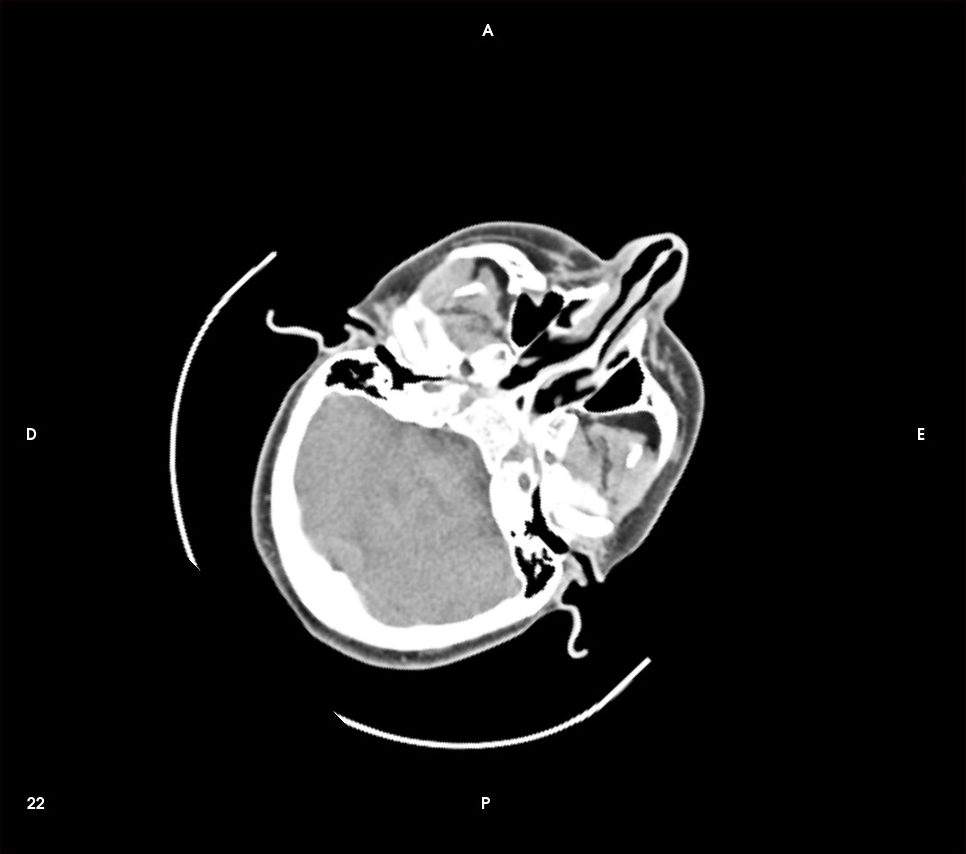
\includegraphics[scale=0.25]{axial_rotate.jpg}
\caption{Imagem rotacionada}
\label{fig:rotate_all}
\end{figure}

\section{Ampliar (\textit{Zoom})}

No InVesalius, existem diferentes formas de ampliar uma imagem. Pode-se maximizar a janela da
orientação desejada, aplicar o \textit{zoom} diretamente na imagem, ou selecionar a região da imagem
que será ampliada.


\subsection{Maximizando as janelas de orientação}

Como já sabemos, a janela principal do InVesalius é dividida em 4 subjanelas: axial, sagital, coronal
e 3D. Cada uma delas pode ser maximizada de modo a ocupar toda a área da janela principal. Para isso,
basta clicar com o botão \textbf{esquerdo} do mouse no ícone existente no \textbf{canto superior direito}
da subjanela (figura \ref{fig:maximize_window}). Para restaurar uma janela maximizada a seu tamanho
anterior, basta clicar novamente no ícone.

\begin{figure}[!htb]
\centering
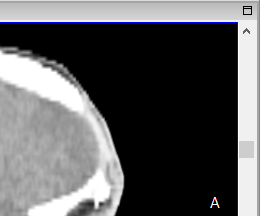
\includegraphics[scale=0.6]{maximize_sagital_mpr.png}
\caption{Detalhe de uma subjanela (Observe o ícone de maximizar no canto superior direito)}
\label{fig:maximize_window}
\end{figure}

\subsection{Ampliando ou reduzindo uma imagem}

Para ampliar ou reduzir uma imagem, clique sobre o ícone do atalho "\textit{Zoom}" na barra de
ferramentas (figura \ref{fig:zoom_icon}). Mantenha o botão \textbf{esquerdo} pressionado sobre
a imagem e \textbf{arraste} o mouse para \textbf{cima}, caso deseje ampliá-la, ou para \textbf{baixo},
caso deseje reduzi-la.

\begin{figure}[!htb]
\centering

\includegraphics[scale=0.25]{tool_zoom_original.png}
\caption{Atalho de \textit{Zoom}}
\label{fig:zoom_icon}
\end{figure}

%\begin{figure}[!htb]
%\centering
%\includegraphics[scale=0.2]{ScreenHunter_76Dec311201_.jpg}
%\caption{Imagem com \textit{Zoom} aplicado}
%\label{fig:zoom_}
%\end{figure}

\subsection{Ampliando uma área da imagem}

Para ampliar uma área determinada da imagem, clique sobre o ícone do atalho "Zoom baseado na seleção" 
na barra de ferramentas (figura \ref{fig:zoom_icon_loc}). Posicione o ponteiro do mouse na posição
inicial da seleção, clique e mantenha o botão \textbf{esquerdo} do mouse pressionado e \textbf{arraste-o}
até a posição final da seleção, formando um retângulo (figura \ref{fig:zoom_select}). Assim que o
botão esquerdo do mouse for liberado, a operação de \textit{zoom} será aplicada à região selecionada
(figura \ref{fig:zoom_applied}).

\begin{figure}[!htb]
\centering

\includegraphics[scale=0.25]{tool_zoom_select_original.png}
\caption{Atalho de \textit{Zoom} baseado na seleção}
\label{fig:zoom_icon_loc}
\end{figure}

\begin{figure}[!htb]
\centering
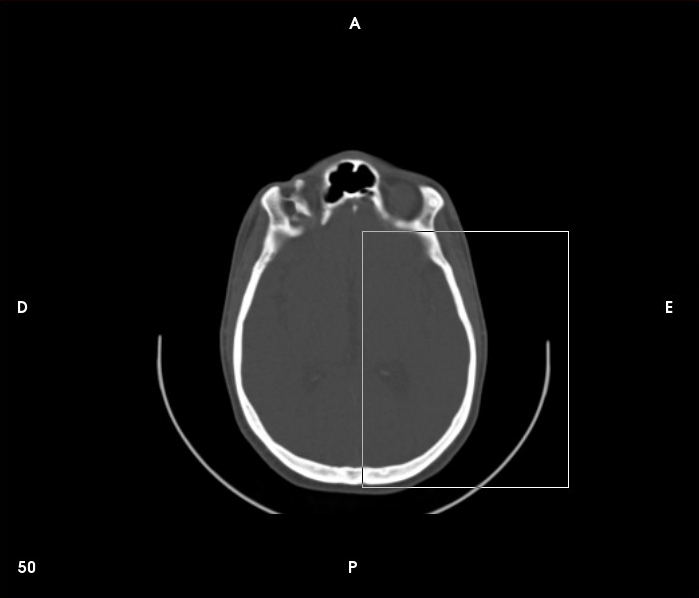
\includegraphics[scale=0.25]{tool_zoom_select_image.jpg}
\caption{Área selecionada para \textit{zoom}}
\label{fig:zoom_select}
\end{figure}

\begin{figure}[!htb]
\centering
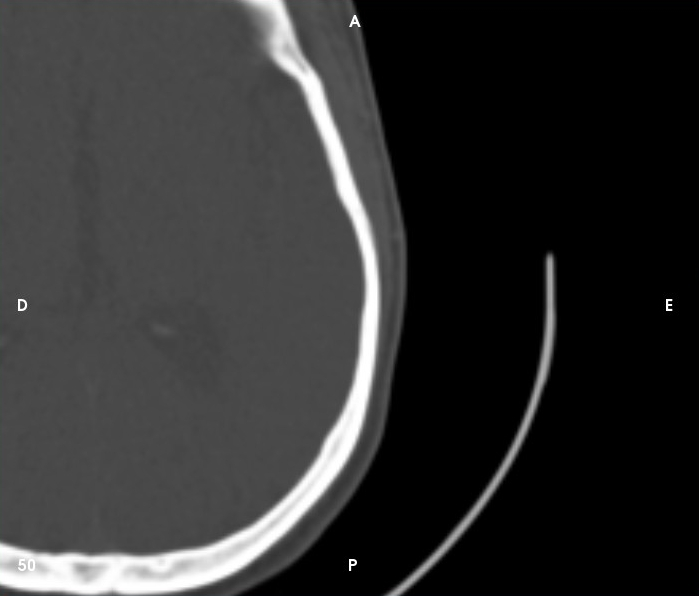
\includegraphics[scale=0.25]{tool_image_with_zoom.jpg}
\caption{Imagem ampliada}
\label{fig:zoom_applied}
\end{figure}


\section{Brilho e contraste (Janelas)}
\label{sec:ww_wl}

Para melhorar a visualização das imagens, podemos utilizar o recurso de \textit{window width} e
\textit{window level}, popularmente conhecido por "brilho e contraste" ou "janela" (para radiologistas). 
Com esse recurso, é possível definir a faixa da escala de cinza (\textit{window level}) e a
largura dessa faixa (\textit{window width}) que serão usadas para exibir as imagens.

O recurso pode ser acionado pelo ícone do atalho "Contraste" na barra de ferramentas. Veja a figura \ref{fig:window_level_shortcut}.

\begin{figure}[!htb]
\centering

\includegraphics[scale=0.70]{tool_contrast_original.png}
\caption{Atalho de brilho e contraste}
\label{fig:window_level_shortcut}
\end{figure}

Para aumentar o brilho, mantenha o botão \textbf{esquerdo} do mouse pressionado e o \textbf{arraste} na 
horizontal para a direita. Para diminuir o brilho, basta arrastar o mouse para a esquerda. O contraste
pode ser alterado arrastando o mouse (com o botão \textbf{esquerdo} pressionado) na vertical: para cima
para aumentar, ou para baixo para diminuir o contraste.

Para desabilitar o recurso, clique novamente sobre o ícone do atalho (figura \ref{fig:window_level_shortcut}).

É possível utilizar padrões pré-definidos de brilho e contraste. A tabela \ref{tab:window_level} relaciona
alguns tipos de tecido com os respectivos valores de brilho e contraste da imagem. Para usar um padrão
pré-definido, posicione o cursor do mouse sobre a imagem e clique com o botão \textbf{direito} para abrir um
menu de contexto sobre ela. Quando o menu se abrir, selecione a entrada \textbf{Brilho e Contraste} e, em
seguida, clique sobre a opção pré-definida, de acordo com o tipo de tecido, como mostra a figura
\ref{fig:window_level}.


\begin{figure}[!htb]
\centering
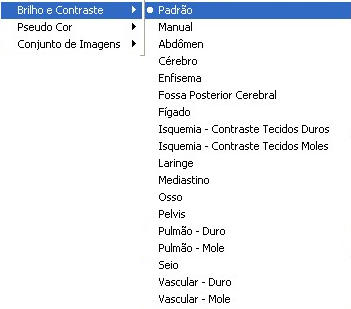
\includegraphics[scale=0.40]{menu_window_and_level_pt.png}
\caption{Menu de contexto para seleção de brilho e contraste}
\label{fig:window_level}
\end{figure}

\begin{table}[h]
\centering
\caption{Valores de brilho e contraste para alguns tecidos}
\begin{tabular}{lcc}\\
\hline % este comando coloca uma linha na tabela
Tecido & Brilho & Contraste\\
\hline
\hline
Padrão & Exame & Exame\\
Manual & Alterado & Alterado\\
Abdômen & 350 & 50 \\
Cérebro & 80 & 40\\
Enfisema & 500 & -850\\
Fossa Posterior Nasal & 120 & 40\\
Fígado & 2000 & -500\\
Isquemia - Contraste Tecidos Duros & 15 & 32\\
Isquemia - Contraste Tecidos Moles & 80 & 20\\
Laringe & 180 & 80\\
Mediastino & 350 & 25\\
Osso & 2000 & 300\\
Pélvis & 450 & 50\\
Pulmão Duro & 1000 & -600\\
Pulmão Mole & 1600 & -600\\
Seio & 4000 & 400\\
Vascular - Duro & 240 & 80\\
Vascular - Mole & 680 & 160\\
\hline
\end{tabular}
\label{tab:window_level}
\end{table} 

\begin{figure}
  \centering
  \subfloat[Osso]{\label{fig:contrast_bone}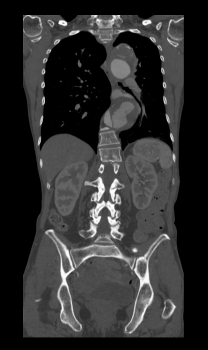
\includegraphics[width=0.4\textwidth]{contraste_osso}}                
  \subfloat[Pulmão]{\label{fig:contrast_isq}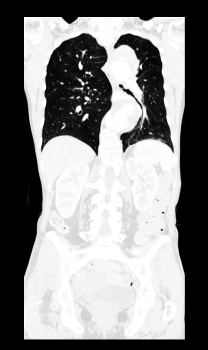
\includegraphics[width=0.4\textwidth]{contraste_pulmao}}
  \caption{Diferentes tipos de brilho e constraste}
  \label{fig:two_window_level}
\end{figure}


\section{Pseudocor}

Outro recurso para melhorar a visualização das imagens são as pseudocores. Elas substituem os níveis
de cinza por cores, ou pelos níveis de cinza invertidos. Nesse último caso, regiões da imagem que
antes eram mais claras se tornam mais escuras e vice-versa.

Para alterar a visualização usando uma pseudocor, posicione o cursor do mouse sobre a imagem e clique
com o botão \textbf{direito} para abrir um menu de contexto sobre ela. Quando o menu se abrir,
selecione a entrada \textbf{Pseudocor} e, em seguida, clique sobre a opção de pseudocor desejada, como
mostra a figura \ref{fig:pseudo_color}.

\begin{figure}[H]
\centering
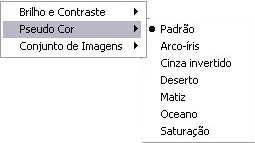
\includegraphics[scale=0.40]{pseudo_menu_pt.png}
\caption{Pseudo Cor}
\label{fig:pseudo_color}
\end{figure}

As figuras de \ref{fig:image_default} a \ref{fig:image_saturation} exemplificam as diversas opções de
pseudocor disponíveis.\\

\begin{figure}[H]
\centering
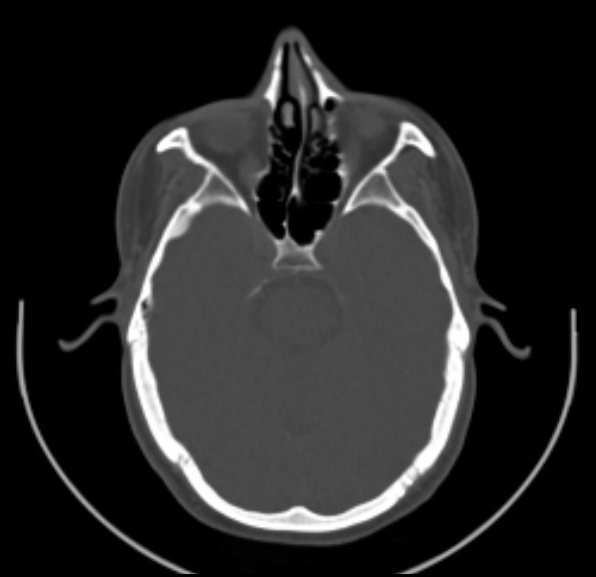
\includegraphics[scale=0.30]{pseudo_default.jpg}
\caption{Padrão}
\label{fig:image_default}
\end{figure}

\begin{figure}[H]
\centering
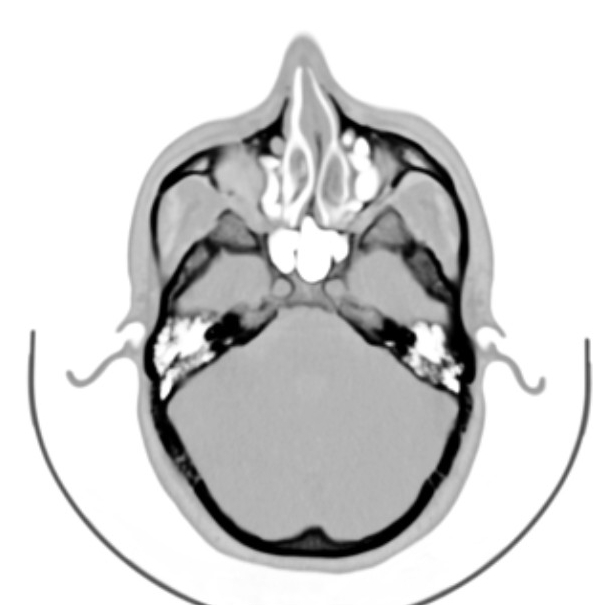
\includegraphics[scale=0.30]{pseudo_inverse.jpg}
\caption{Imagem Cinza Invertido}
\label{fig:image_inverted}
\end{figure}

\begin{figure}[H]
\centering
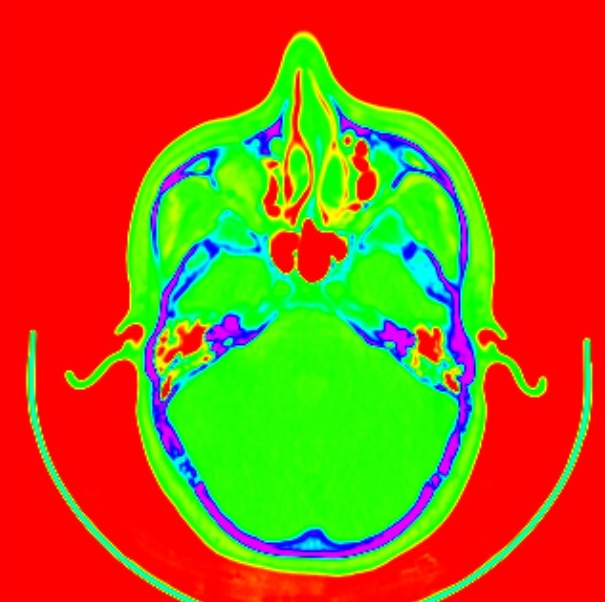
\includegraphics[scale=0.30]{pseudo_rainbow.jpg}
\caption{Arco-íris}
\label{fig:image_arc}
\end{figure}

\begin{figure}[H]
\centering
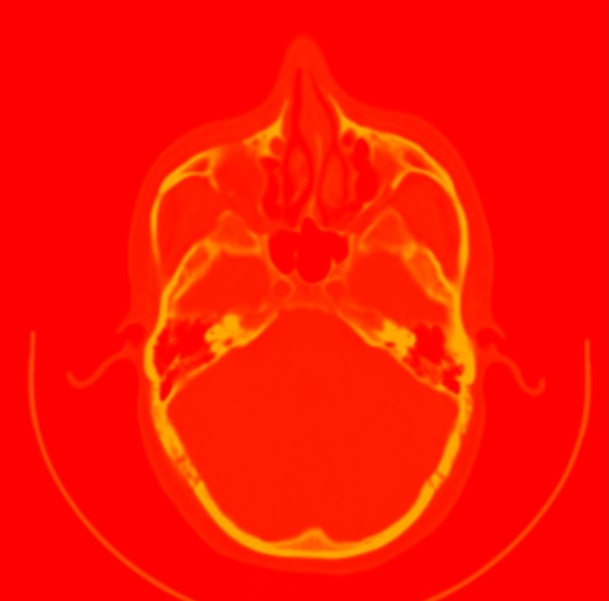
\includegraphics[scale=0.30]{pseudo_desert.jpg}
\caption{Deserto}
\label{fig:image_desert}
\end{figure}

\begin{figure}[H]
\centering
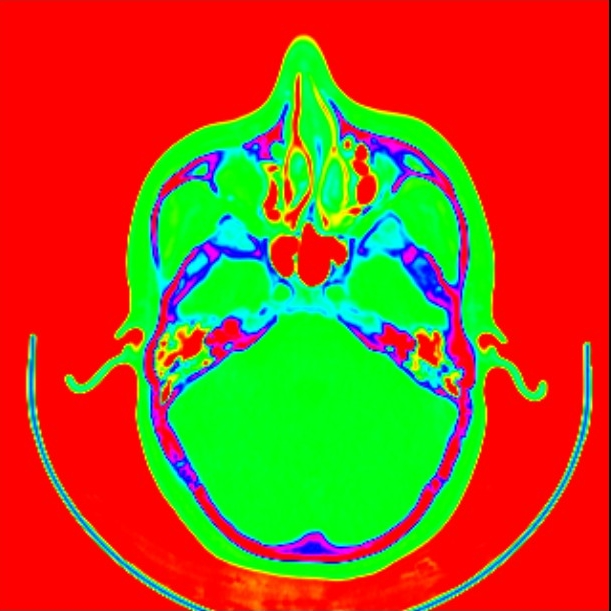
\includegraphics[scale=0.30]{pseudo_hue.jpg}
\caption{Matiz}
\label{fig:image_matiz}
\end{figure}

\begin{figure}[H]
\centering
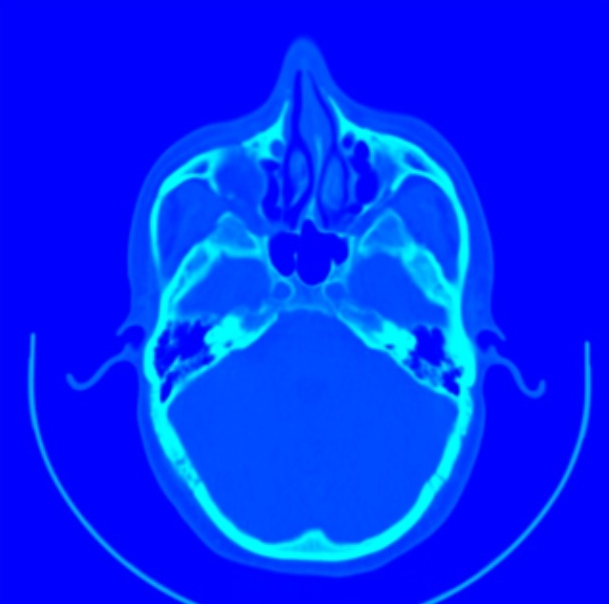
\includegraphics[scale=0.30]{pseudo_ocean.jpg}
\caption{Oceano}
\label{fig:image_ocean}
\end{figure}

\begin{figure}[H]
\centering
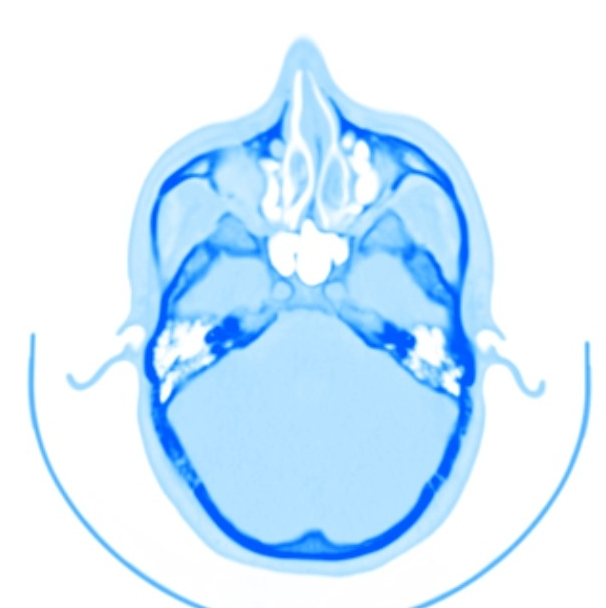
\includegraphics[scale=0.30]{pseudo_saturation.jpg}
\caption{Saturação}
\label{fig:image_saturation}
\end{figure}

\newpage

\section{Tipo de projeção}

É possível alterar o tipo de projeção das imagens 2D a serem visualizadas, além do modo normal, o InVesalius dispõe de seis tipos de projeções que podem serem acessadas da seguinte forma: Possicione o cursor do mouse sobre a imagem e clique com o botão \textbf{direito} para abrir um menu de contexto sobre ela. Quando o menu se abrir, selecione a entrada tipo de projeção e, em seguida, clique sobre a opção de pseudocor desejada, como mostra a figura~\ref{fig:menu_proj}.

\begin{figure}[H]
\centering
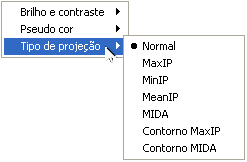
\includegraphics[scale=0.60]{menu_projection_pt.png}
\caption{Menu de Tipo de projeção}
\label{fig:menu_proj}
\end{figure}

\subsection{Normal}

O modo normal é a visualização padrão, ou seja, sem nenhum tipo de projeção, da maneira em que a imagem foi adquirida ou customizada previamente seja com brilho e contraste ou pseudocor. Exemplificamos na figura~\ref{fig:proj_normal}.

\begin{figure}[H]
\centering
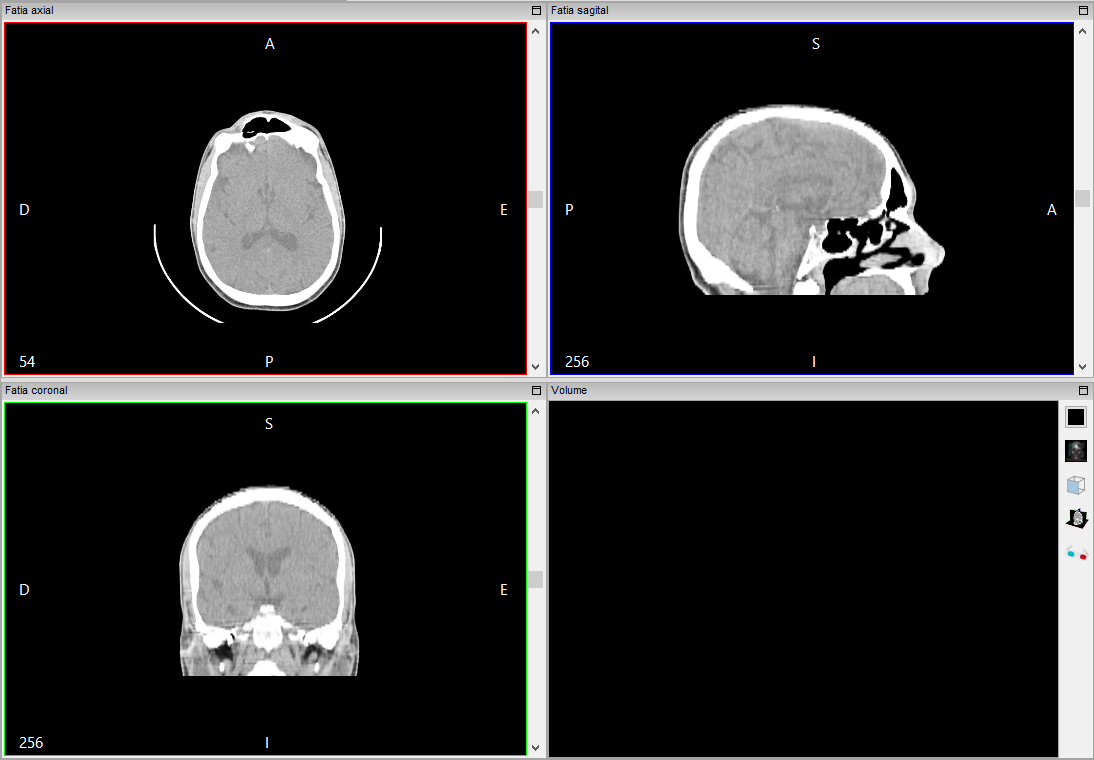
\includegraphics[scale=0.40]{multiplanar_window_pt.png}
\caption{Projeção normal}
\label{fig:proj_normal}
\end{figure}

\subsection{MaxIP}
\label{sec:max_ip}
MaxIP também é conhecido como MIP (\textit{Maximum Intensity Projection}), o método seleciona somente os voxels que possuem intensidade máxima entre os visitados como mostra a figura~\ref{fig:proj_maxip}. De acordo com a quantidade ou "profundidade" do MaxIP cada voxel é visitado em ordem de sobreposição, por exemplo, para selecionar MaxIP do pixel $(0,0)$ composto por 3 fatias é necessário visitar o pixel $(0,0)$ das fatias $(1,2,3)$ e selecionar o maior valor.

\begin{figure}[H]
\centering
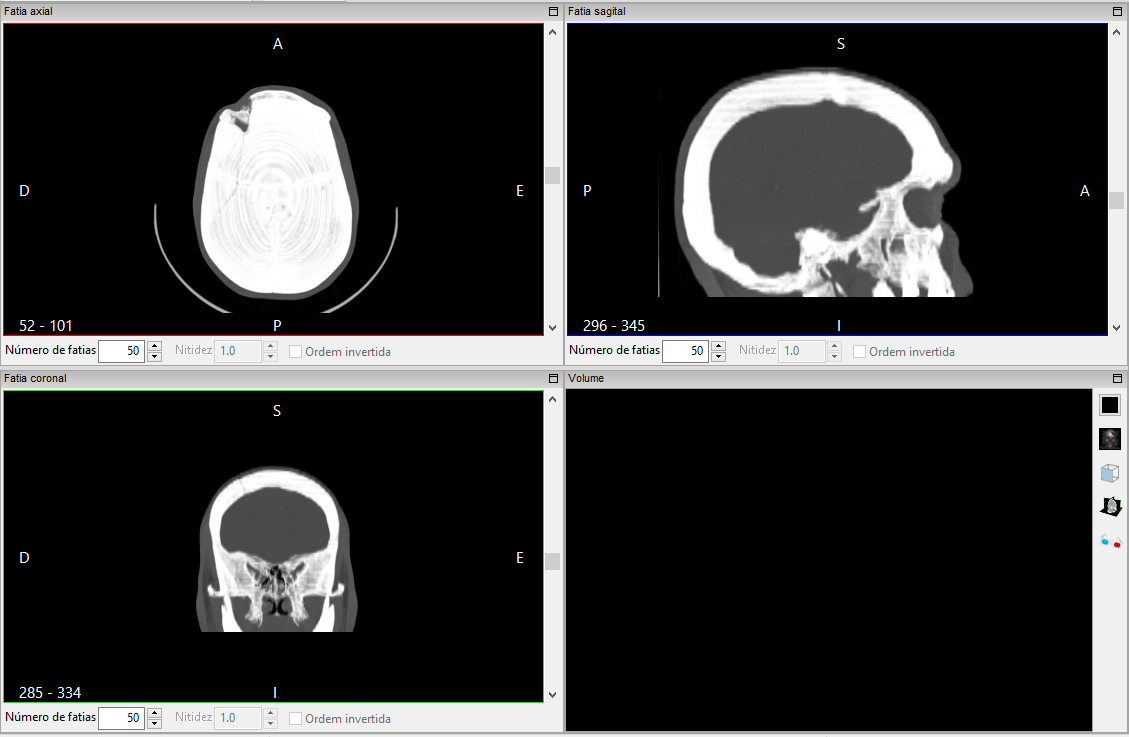
\includegraphics[scale=0.40]{multiplanar_window_maxip_pt.png}
\caption{Projeção MaxIP ou MIP}
\label{fig:proj_maxip}
\end{figure}

Como mostra a figura~\ref{fig:proj_maxip_qtd}, a quantidade de imagens que irá compor o MaxIP é setada no inferior da imagem de cada orientação.

\begin{figure}[H]
\centering
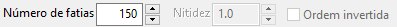
\includegraphics[scale=0.80]{multiplanar_window_maxip_number_pt.png}
\caption{Seleção da quantidade de imagens que compõe o MaxIP ou MIP}
\label{fig:proj_maxip_qtd}
\end{figure}

\subsection{MinIP}

Ao contrário do MaxIP, o MinIP (\textit{Minimun Intensity Projection}) seleciona somente os voxels que possuem internsidade minima entre os visitados, apresentamos na figura~\ref{fig:proj_minIP} um exemplo. A seleção da quantidade de imagens que irá compor a projeção é feita no inferior da imagem de cada orientação como mostra a figura~\ref{fig:proj_maxip_qtd}.

\begin{figure}[H]
\centering
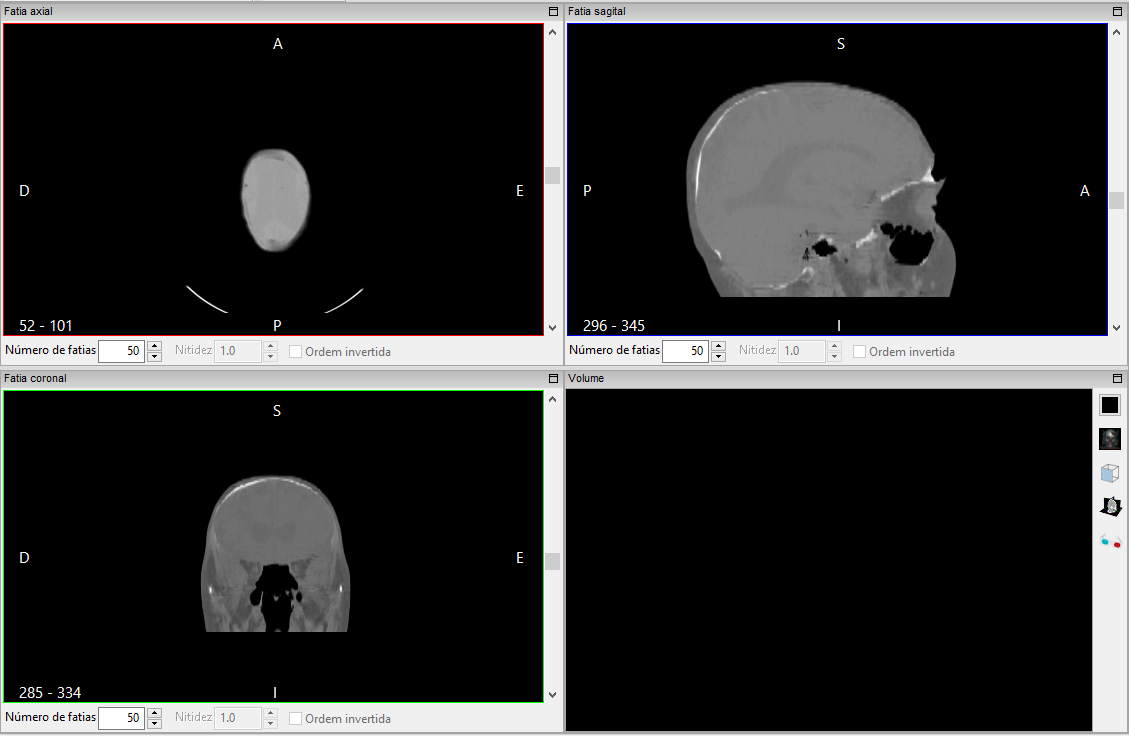
\includegraphics[scale=0.40]{multiplanar_window_minip_pt.png}
\caption{Projeção MinIP}
\label{fig:proj_minIP}
\end{figure}

\subsection{MeanIP}
A técnica MeanIP (\textit{Mean Intensity Projection}) que é mostrada na figura~\ref{fig:proj_meanIP} compõe a projeção realizando a média dos voxels visitados. Os voxels são visitados da mesma forma dos métodos MaxIP e MinIP. Também é possível definir quantas imagens irão compor a projeção no inferior da imagem de cada orientação como é mostrada na figura~\ref{fig:proj_maxip_qtd}.

\begin{figure}[H]
\centering
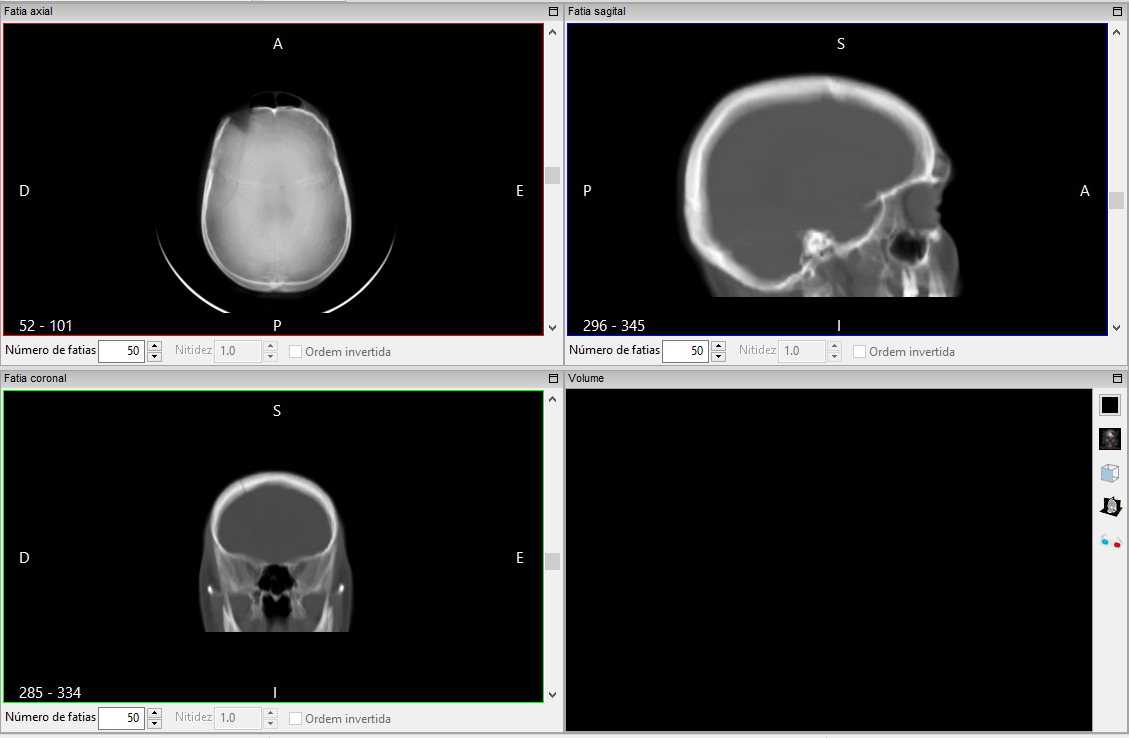
\includegraphics[scale=0.40]{multiplanar_window_mean_pt.png}
\caption{Projeção MeanIP}
\label{fig:proj_meanIP}
\end{figure}

\subsection{MIDA}
\label{sub:mida}
A técnica MIDA (\textit{Maximum Intensity Difference Accumulation}) projeta uma imagem levando em consideração somente os voxels que possuem valores máximos locais. A partir de cada pixel da tela é simulado um raio em direção ao volume, cada voxel é interceptado por cada um destes raios chegando até o final do volume, cada um desses voxels visitados tem o seu valor acumulado, mas são levados em consideração somente se o valor for maior que os valores já visitados anteriormente. A exemplo do MaxIP, é possível selecionar quantas imagens serão utilizadas para acumular os valores. Apresentamos na figura~\ref{fig:proj_MIDA} um exemplo de projeção MIDA.  

\begin{figure}[H]
\centering
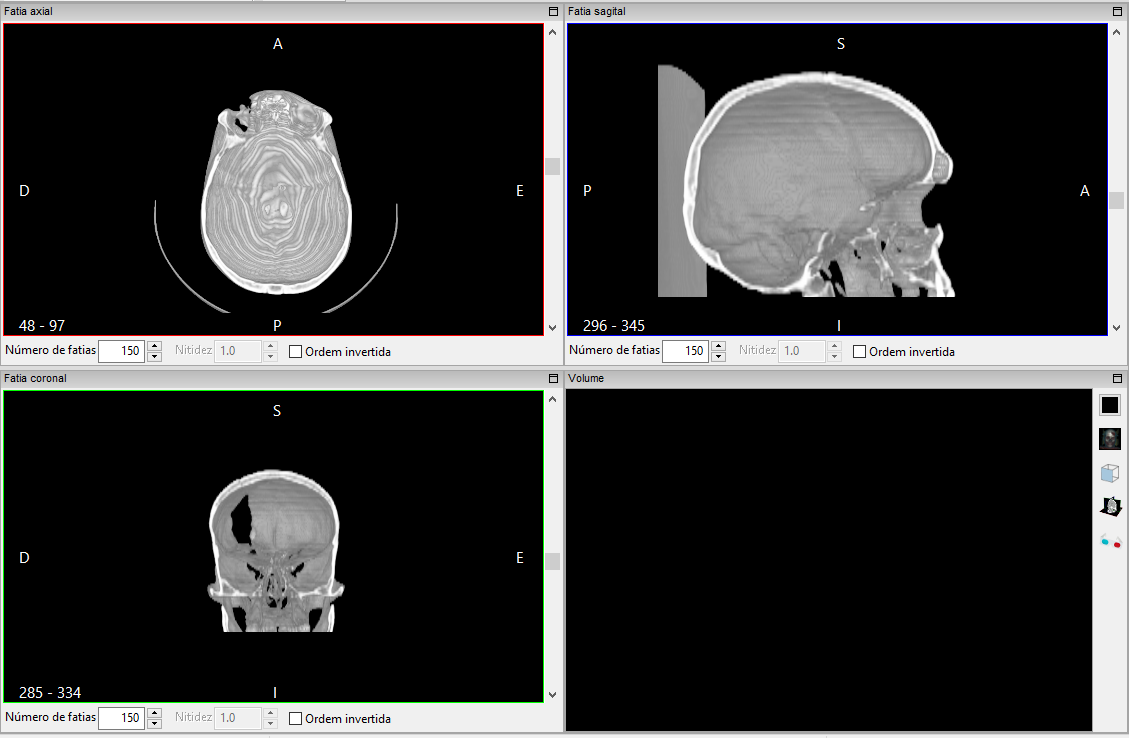
\includegraphics[scale=0.40]{multiplanar_window_mida_pt.png}
\caption{Projeção MIDA}
\label{fig:proj_MIDA}
\end{figure}

Como mostra a figura~\ref{fig:proj_MIDA_inv}, é possível inverter a ordem que os voxels são visitados, bastando selecionar a opção \textbf{Ordem invertida} no canto inferior da tela.

\begin{figure}[H]
\centering
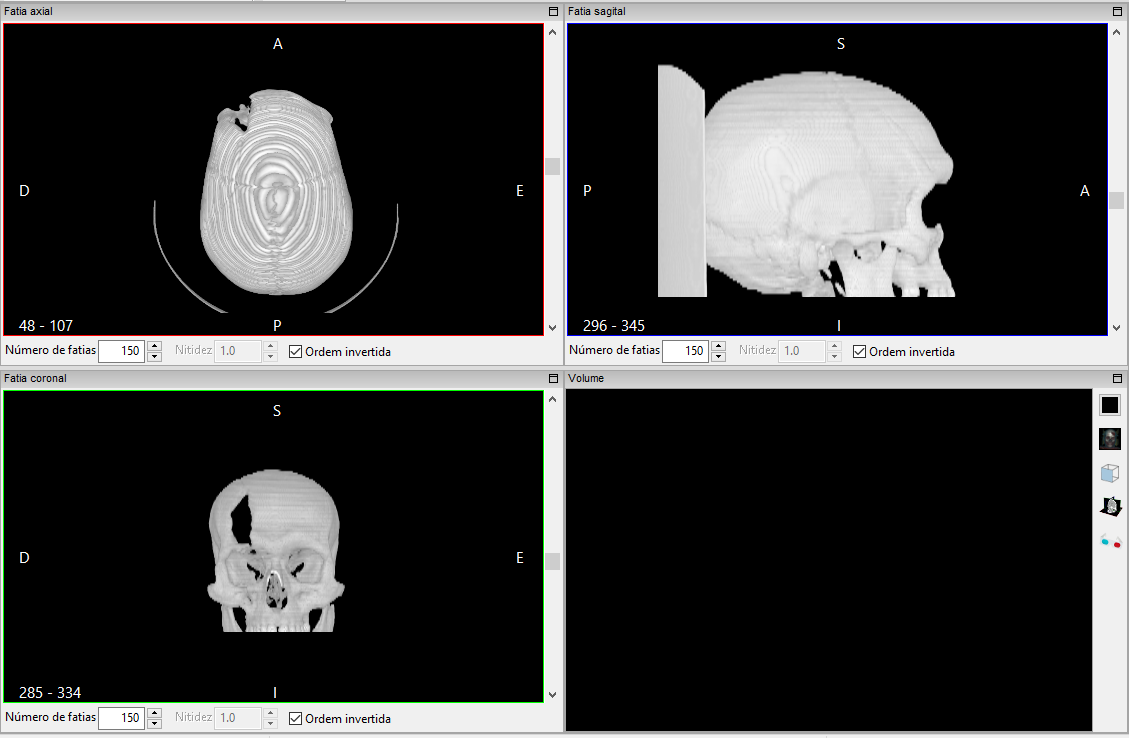
\includegraphics[scale=0.40]{multiplanar_window_mida_inverted_pt}
\caption{Projeção MIDA em ordem invertida}
\label{fig:proj_MIDA_inv}
\end{figure}

\subsection{Contorno MaxIP}

Compõe a projeção 2D do conjunto de imagens que contém o volume usando a técnica \textit{Contour MaxIP}. A técnica consiste em visualizar contornos presentes na projeção gerada com a técnica MaxIP(\ref{sec:max_ip}). Um exemplo é apresentado na figura~\ref{fig:proj_contorno_maxip}.

\begin{figure}[H]
\centering
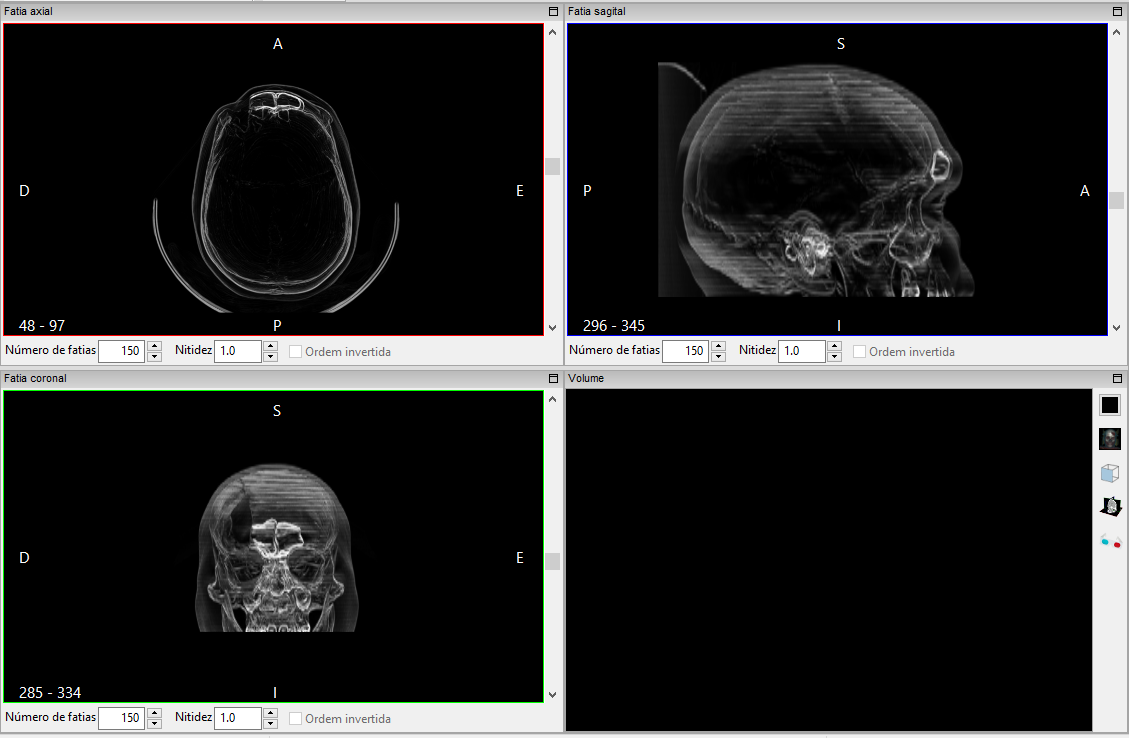
\includegraphics[scale=0.40]{multiplanar_window_contour_maxip_pt.png}
\caption{Projeção de Contorno MaxIP}
\label{fig:proj_contorno_maxip}
\end{figure}

\subsection{Contorno MIDA}

Compõe a projeção 2D do conjunto de imagens que contém o volume usando a técnica \textit{Contour MIDA}. A técnica consiste em visualizar contornos presentes na projeção gerada com a técnica MIDA(\ref{sub:mida}). A exemplo do MIDA é possível inverter a ordem que o volume é visitado. Exemplificamos na figura~\ref{fig:proj_contorno_mida}.

\begin{figure}[H]
\centering
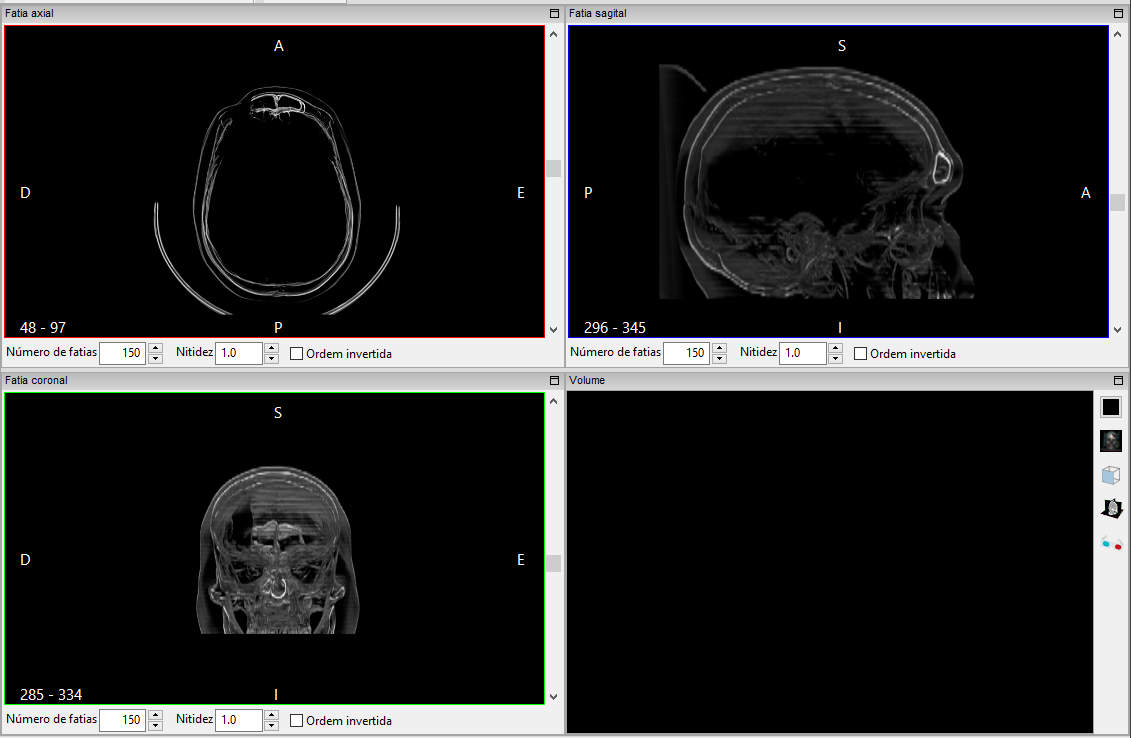
\includegraphics[scale=0.40]{multiplanar_window_contour_mida_pt.png}
\caption{Projeção de Contorno MIDA}
\label{fig:proj_contorno_mida}
\end{figure}